\subsection{Exploratory Data Analysis}

\qquad To figure out if there are any questions that can determine the dialect geography patterns, we pick out 3 questions to look into, i.e. \textit{Question 74}, \textit{Question 76} and \textit{Question 89}. The contents are displayed as followings: 

\begin{itemize}
\item Q074: What do you call the little gray creature (that looks like an insect but is actually a crustacean) that rolls up into a ball when you touch it?
   
\item Q076:  What term do you use to refer to something that is across both streets from you at an intersection (or diagonally across from you in general)?

\item Q089: Can you call coleslaw "slaw"?
\end{itemize}

\qquad These three questions focus on the way people call several common stuffs. \textit{Question 74} has 14 choices, \textit{Question 76} has 9 and \textit{Question 89} has 5, which reflects the diversity of dialects. \textit{Question 76} and \textit{Qeustion 89} share a similar pattern that they separate the southern interviewees from the others, while \textit{Question 74} isolates the northern part and eastern part (See \href{https://yeyt2718.shinyapps.io/map_Question}{Map Set} for the map distribution based on questions). It's easy to interpret the isolated eastern and northern part with responses like 'no idea' as the cold environment offer them few opportunities of seeing such bugs. But other questions may involve complicated cultural and historical factors.\\




\qquad  We further try to find out if there exists obvious association between different questions. The correlation of the pairwise questions is calculated by performing a kernel density estimation on the two dimension distribution (e.g., $Q074 \times Q076$), as shown in \textbf{Figure \ref{fig:question distribution}}. Most people incline to response 'roly poly' to \textit{Question 74} and 'kitty-conner' to\textit{Question 76} simultaneously or take 'roly poly' and 'catty corner' as a pari. Such connection can help predict the response for each other. No meaningful information can be extracted by looking at the 2D density estimation between \textit{Question 74} and \textit{Question 89} or between \textit{Question 76} and \textit{Question 89}. It just indicates that we should not only focus one or two questions to detect the dialect geography, but should aggregate all of them for analysis \textbf{[reference!]}. Motivated by this, we move on implementing clustering methods based on all the 67 questions.



\begin{figure*}[t!]
%  \begin{minipage}[b]{0.49\textwidth}
%    \centering
%    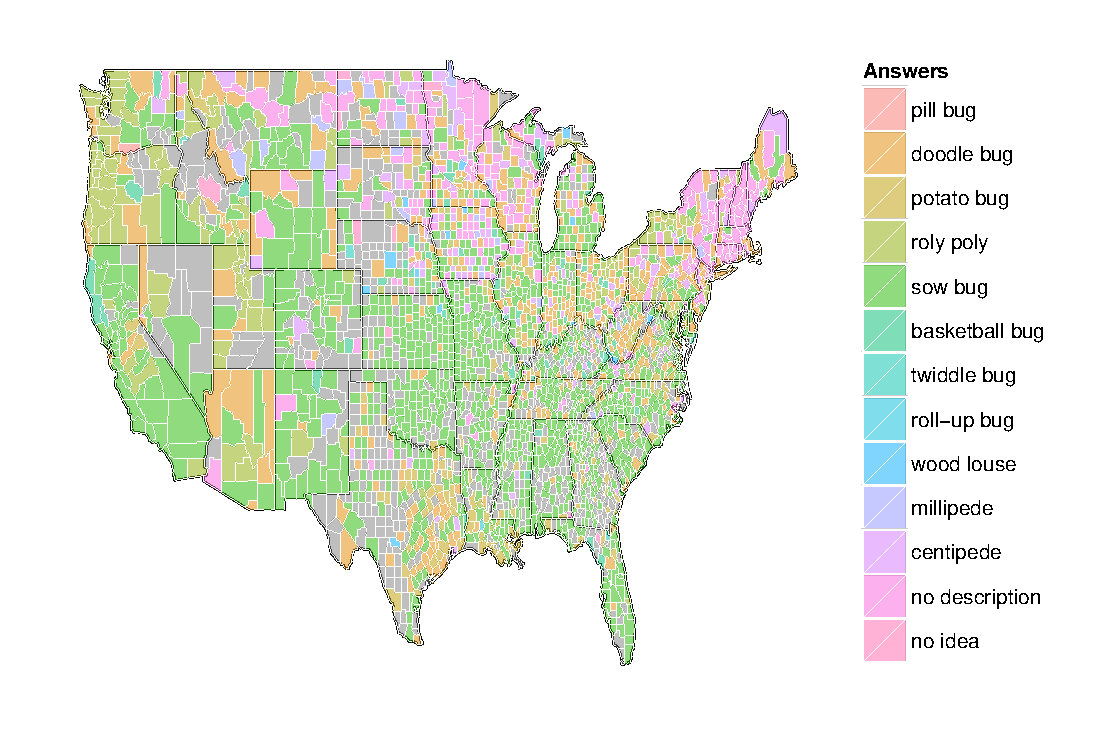
\includegraphics[width=1.1\columnwidth,height=0.7\columnwidth]{fig/Map_Q74.pdf}
%    \subcaption{Question 74}\label{subfig:hierarchy1}
%  \end{minipage}
  \begin{minipage}[t]{0.33\textwidth}
    \centering
    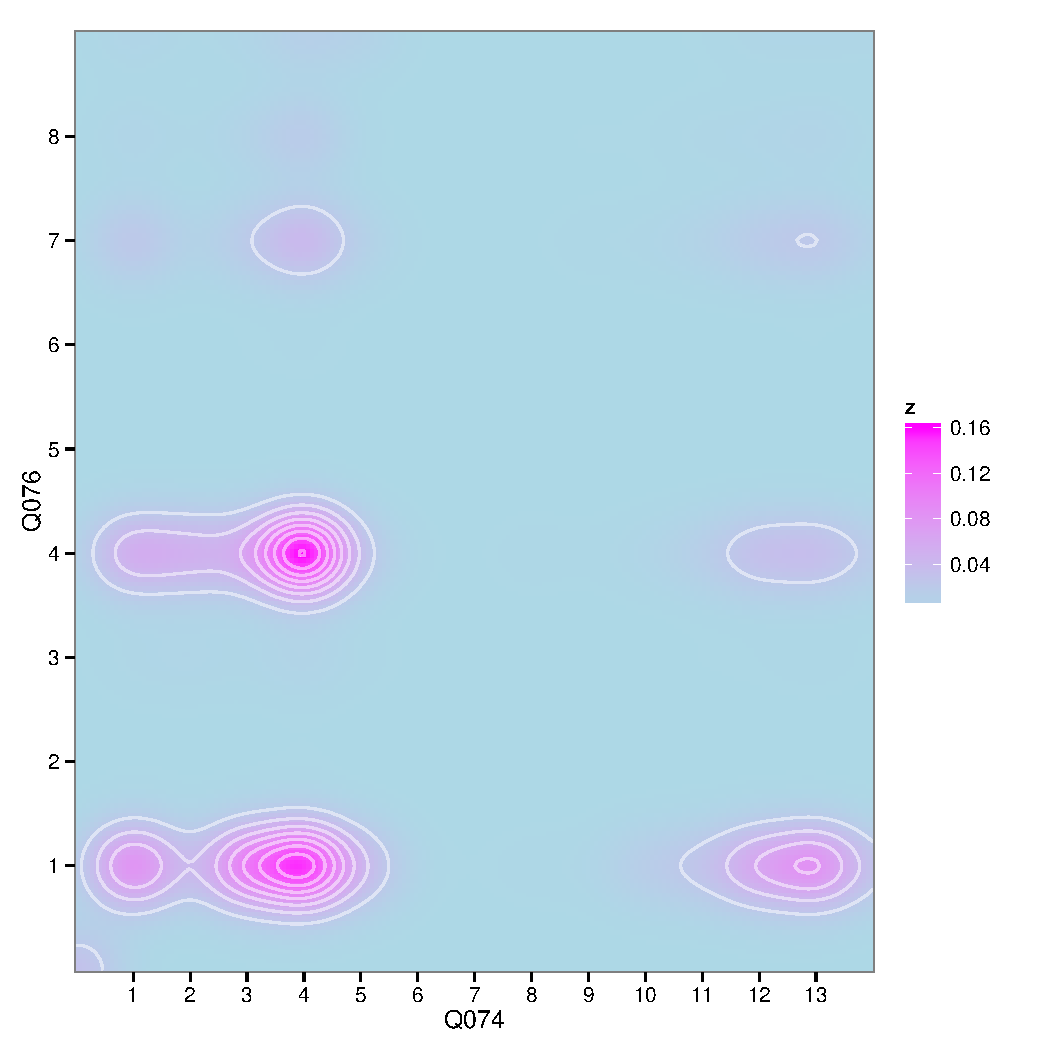
\includegraphics[width=\columnwidth,height=0.8\columnwidth]{fig/2dhist_q074_q076.pdf}
    \subcaption{Q074 and Q076}\label{subfig:hierarchy2}
  \end{minipage}
%  \begin{minipage}[b]{0.49\textwidth}
%    \centering
%    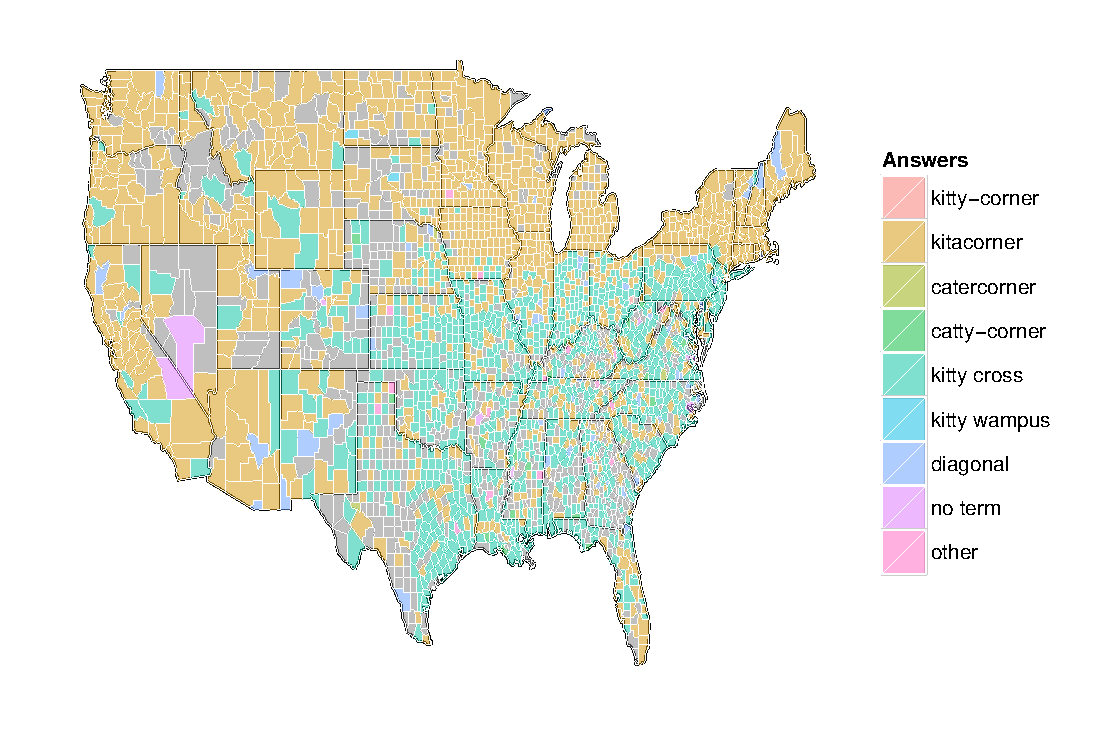
\includegraphics[width=1.1\columnwidth,height=0.7\columnwidth]{fig/Map_Q76.pdf}
%    \subcaption{Question 76}\label{subfig:hierarchy3}
%  \end{minipage}
  \begin{minipage}[t]{0.33\textwidth}
    \centering
    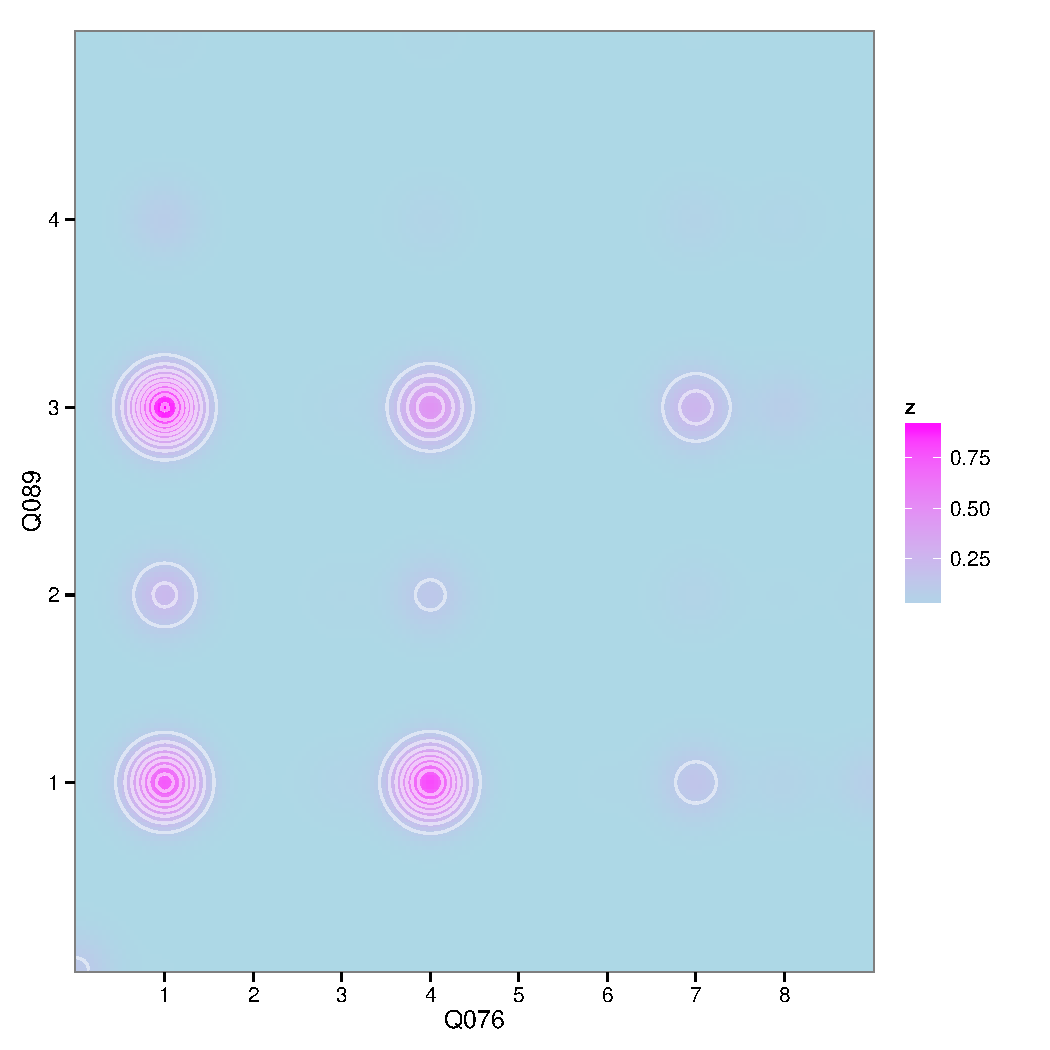
\includegraphics[width=\columnwidth,height=0.8\columnwidth]{fig/2dhist_q076_q089.pdf}
    \subcaption{Q076 and Q089}\label{subfig:hierarchy4}
  \end{minipage}
%  \begin{minipage}[b]{0.49\textwidth}
%    \centering
%    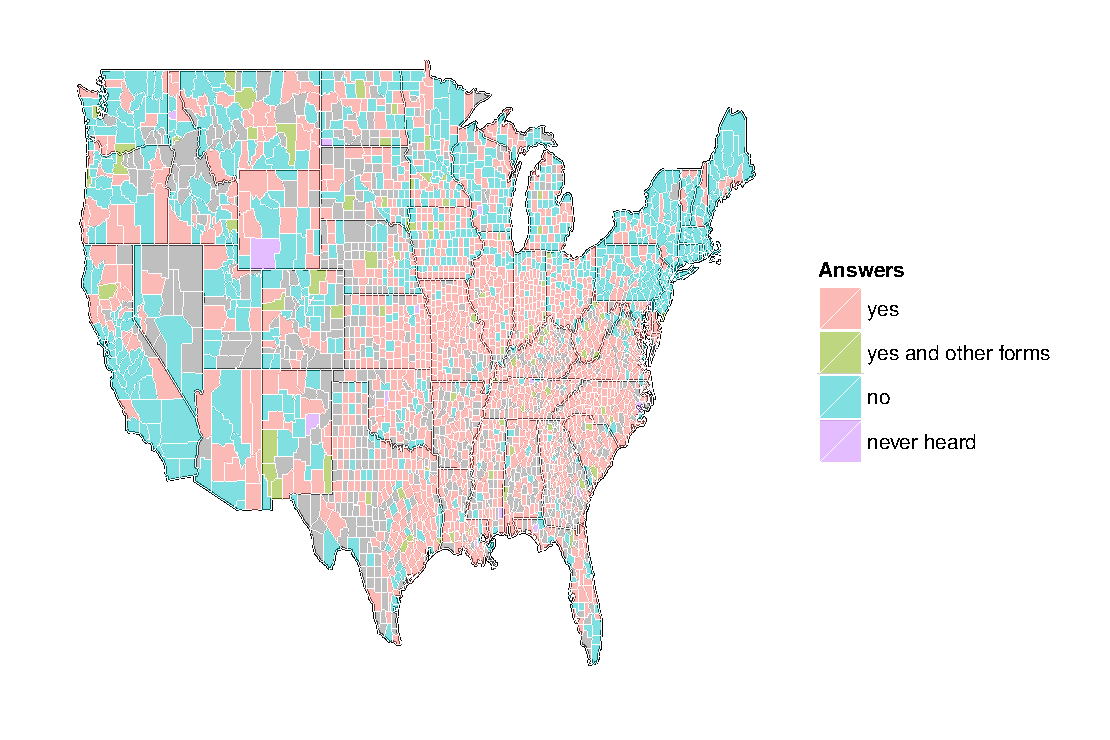
\includegraphics[width=1.1\columnwidth,height=0.7\columnwidth]{fig/Map_Q89.pdf}
%    \subcaption{Question 89}\label{subfig:hierarchy6}
%  \end{minipage}
  \begin{minipage}[t]{0.36\textwidth}
    \centering
    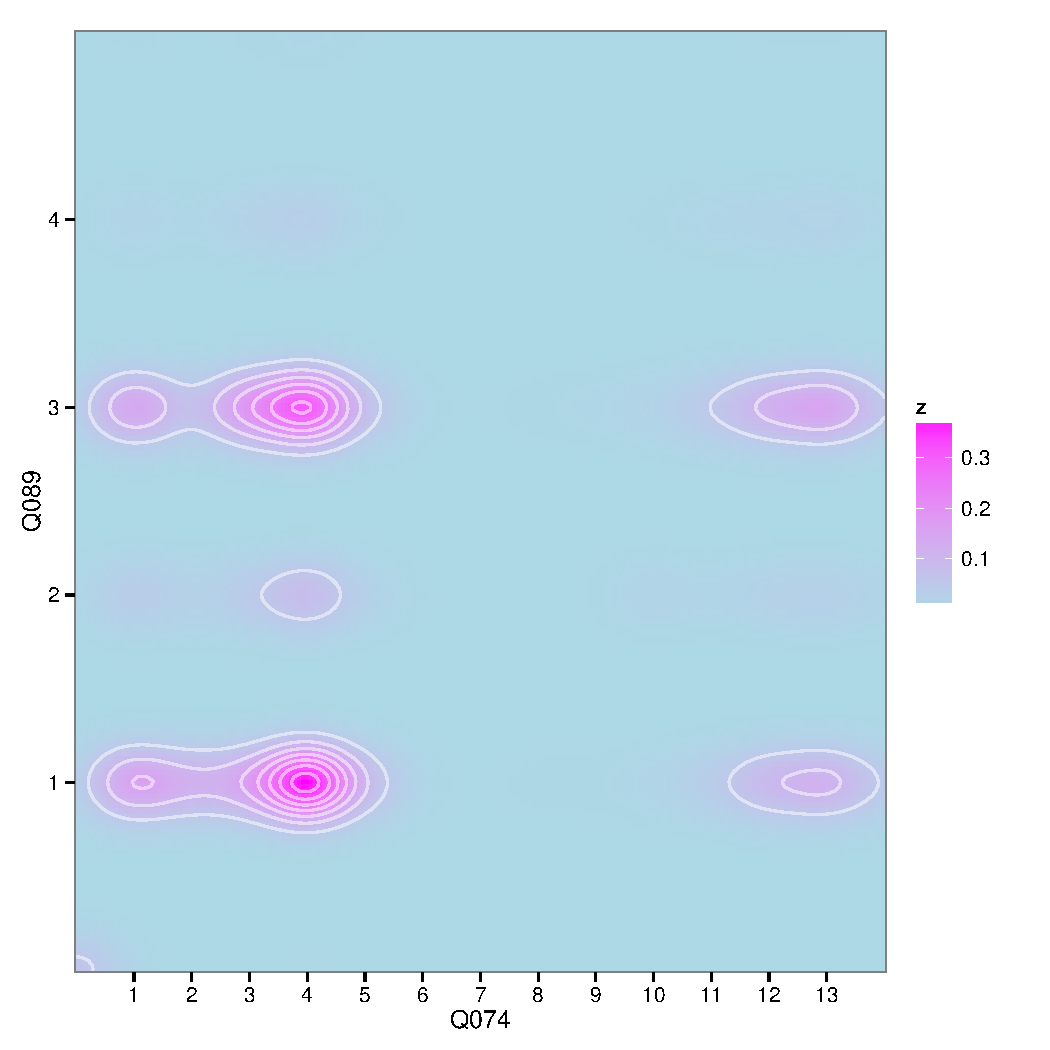
\includegraphics[width=\columnwidth,height=0.8\columnwidth]{fig/2dhist_q074_q089.pdf}
    \subcaption{Q074 and Q089}\label{subfig:hierarchy}
  \end{minipage}
  \caption{\textbf{Pairwise 2D Kernel densitiy estimation.}}
  \label{fig:question distribution}
\end{figure*}


%\begin{figure}[t!]
%    \centering
%    \begin{subfigure}[t]{0.49\textwidth}
%        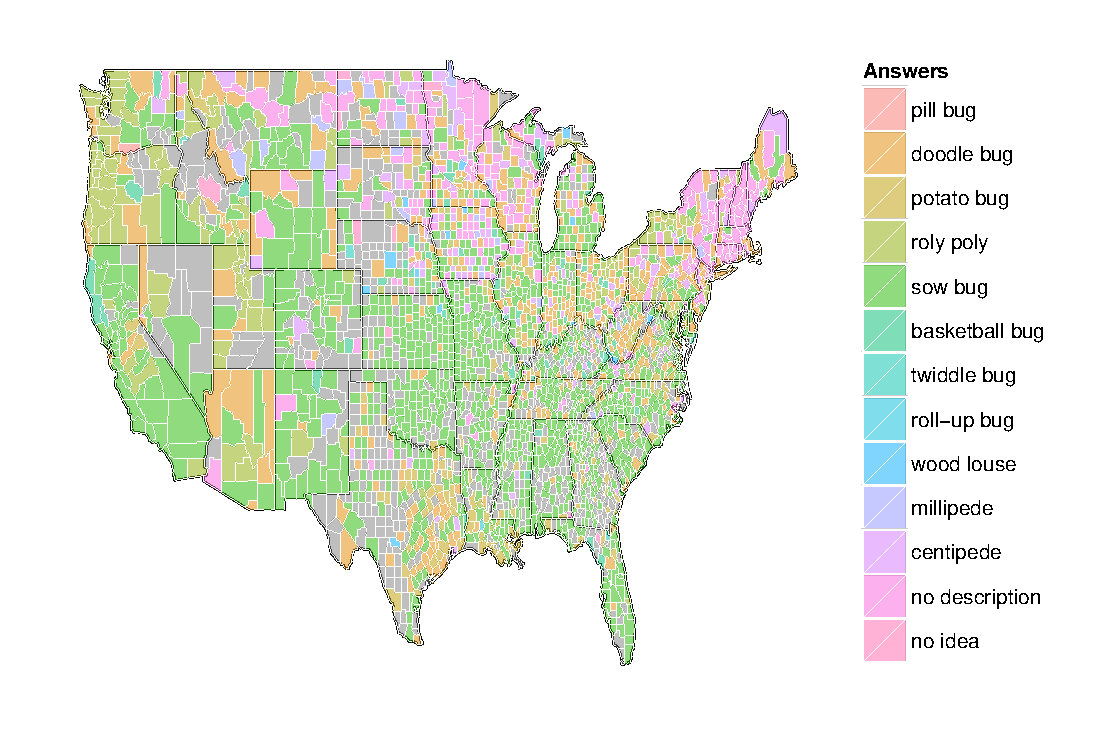
\includegraphics[width=1.1\textwidth]{fig/Map_Q74}
%        \caption{Question 74}
%    \end{subfigure}
%    \begin{subfigure}[t]{0.49\textwidth}
%        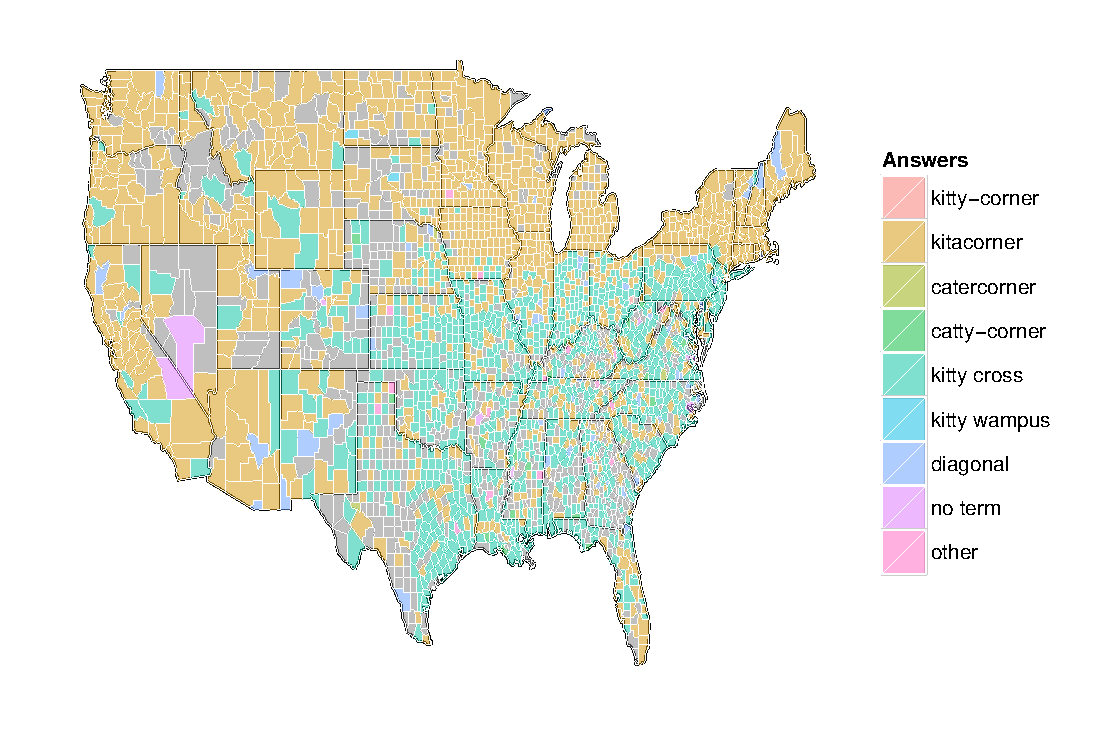
\includegraphics[width=1.1\textwidth]{fig/Map_Q76}
%        \caption{Question 76}
%    \end{subfigure}
%    \caption{\textbf{Answer distribution} \textbf{(a)} Q74. \textbf{(b)} Q76.} 
%\end{figure}

%\noindent In order to quantify the correlation of the two questions (Q074 and Q076), we performed a %kernel density estimation on
%the two dimension distribution ($Q074 \times Q076$), as shown in Figure xx. One see a clear %correlation from the heatmap plotting.\\

%\begin{figure}
%\centering
%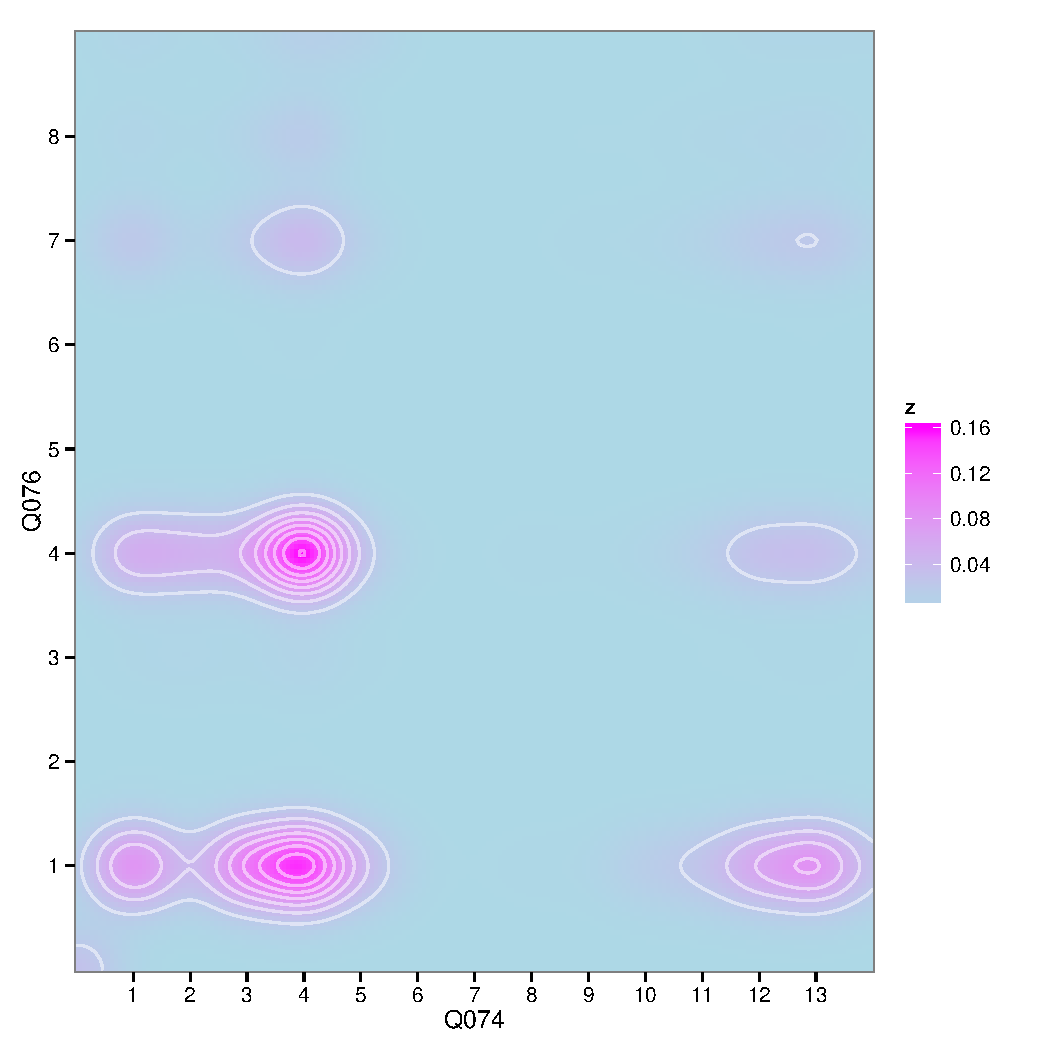
\includegraphics[width=0.45\linewidth]{fig/2dhist_q074_q076}
%\caption{Kernel density estimation for Q074 and Q096}
%\end{figure}

%\noindent Considering more then two questions, we involved Q089, which also share a similar trend %with Q076 and Q074. See Figure xx for the distribution of Q089. And also, we plot two-dimensional %kernel density estimation for two pairs (Q076 vs Q089, Q074 vs Q089), as shown in
%Figure xx.

%\begin{figure}
%\centering
%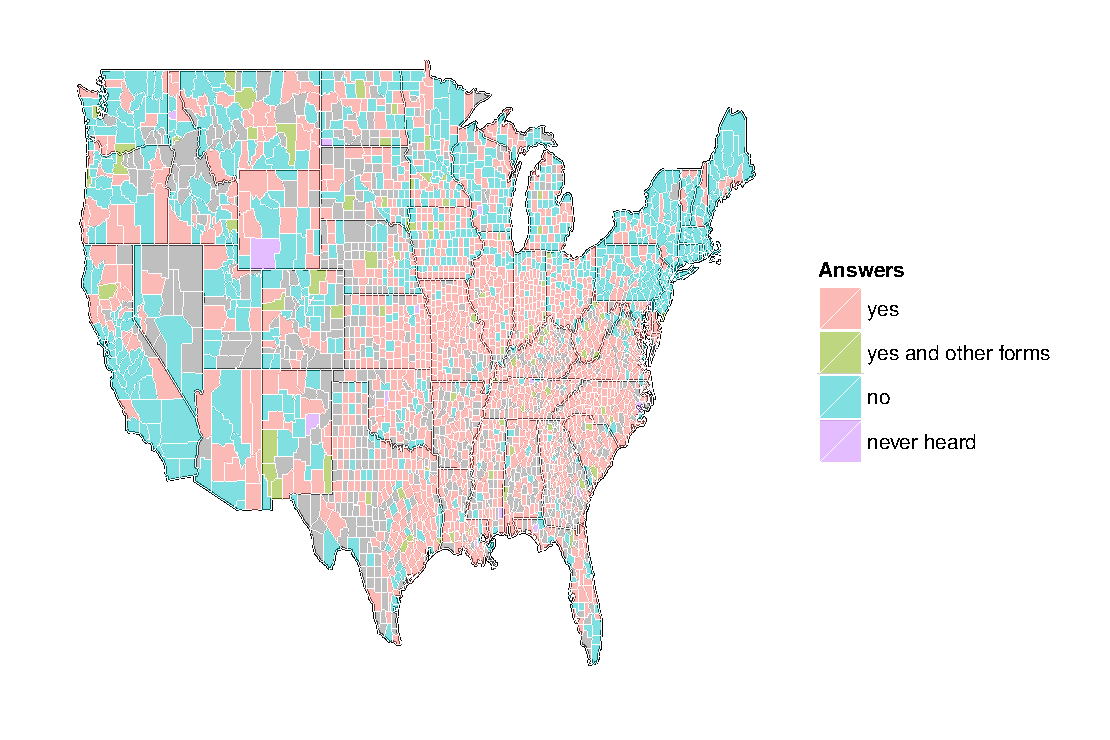
\includegraphics[width=0.9\linewidth]{fig/Map_Q89}
%\caption{Answer Distribution for Q089}
%\end{figure}


%\begin{figure}[t!]
%    \centering
%    \begin{subfigure}[t]{0.49\textwidth}
%        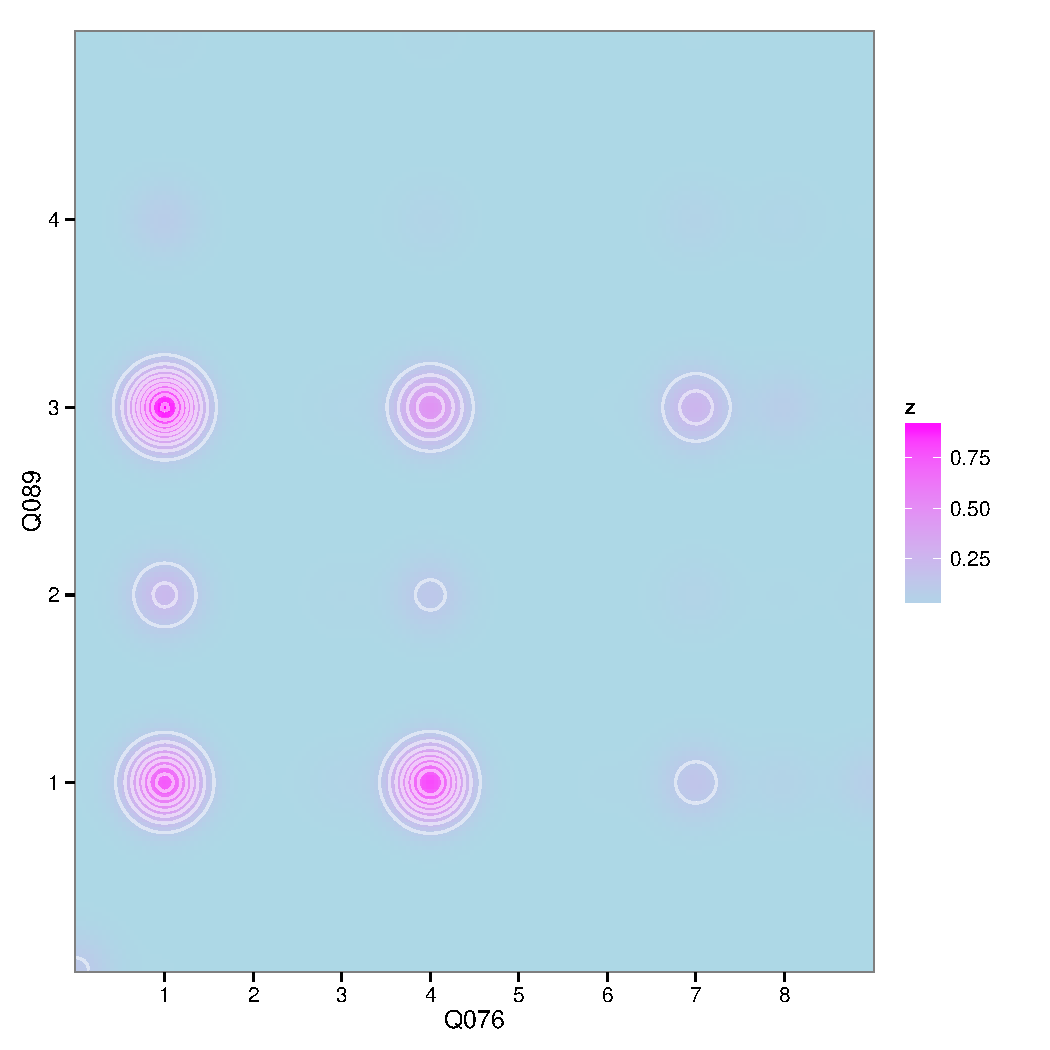
\includegraphics[width=1.1\textwidth]{fig/2dhist_q076_q089}
%        \caption{Q076 .vs. Q089}
%    \end{subfigure}
%    \begin{subfigure}[t]{0.49\textwidth}
%        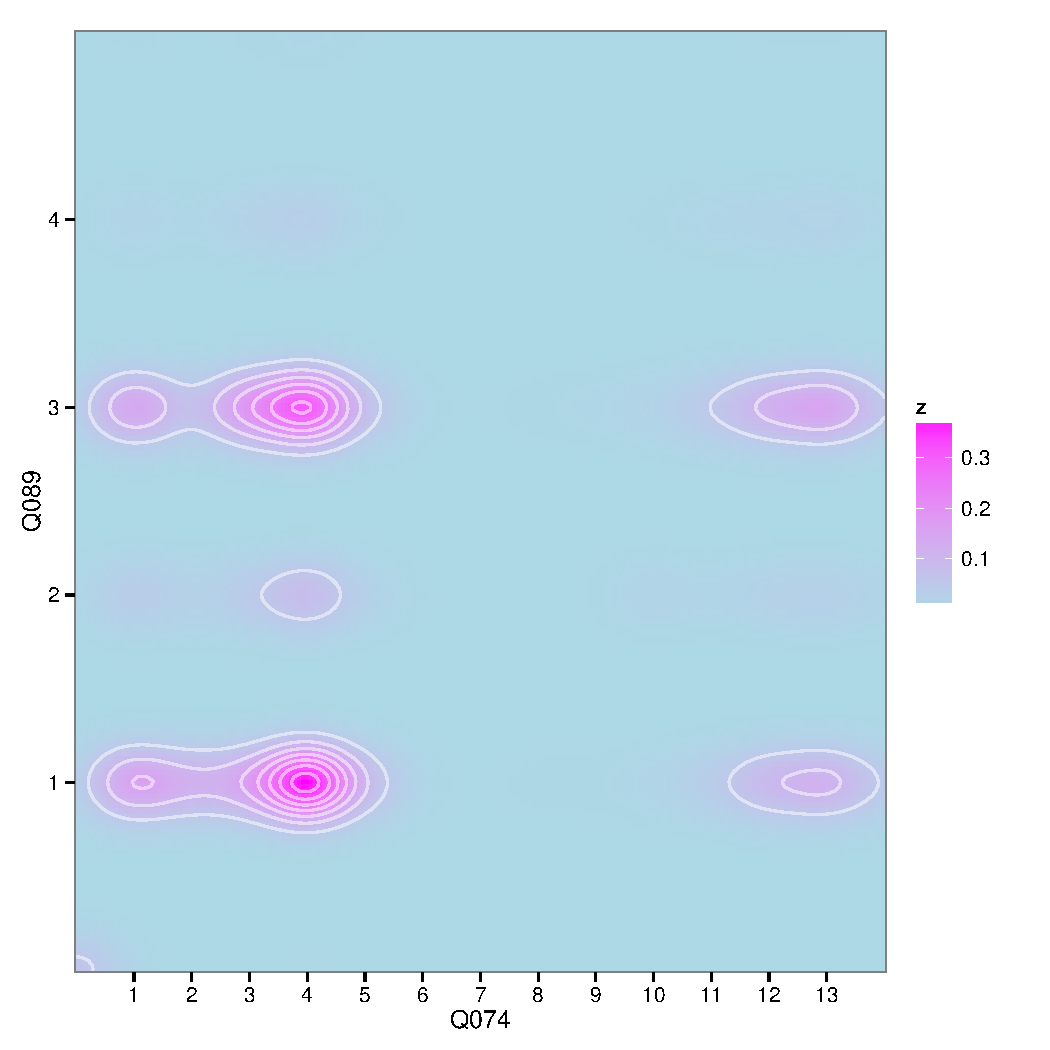
\includegraphics[width=1.1\textwidth]{fig/2dhist_q074_q089}
%        \caption{Q074 .vs. Q089}
%    \end{subfigure}
%    \caption{\textbf{Kernel Density Estimation} \textbf{(a)} Q76 .vs. Q089 \textbf{(b)} Q74 .vs. %Q089} 
%\end{figure}
